\chapter{Internship Context}
\label{chap:premierchapitre}
\section*{Internship Context}
This opening chapter focuses on introducing the host company STMicroelectronics, and provides an overview of the company's activities and global presence. It also includes an introduction to ST Tunis and the Support Solutions team, which played a pivotal role in the execution of this project, as well as an outline of the project's overall framework. Following the presentation of the challenges, we will explore the current state of the art and finally present the proposed solution which is the main objective of this project.

\section{Host Organization}
\subsection{STMicroelectronics}

STMicroelectronics (ST) is a global leader in the semiconductor industry, providing innovative solutions across various markets, including automotive, industrial, personal electronics, and communications equipment.

Founded in 1987 through the merger of SGS Microelettronica of Italy and Thomson Semiconducteurs of France, ST has grown to become one of the largest semiconductor companies in the world.

\subsection{Activity Sectors}

ST's mission is to be the undisputed leader in the semiconductor market, delivering sustainable and innovative solutions that make a positive impact on people's lives. The company's vision is to create technology that enables a more intelligent and connected world, driving progress in key areas such as smart driving, smart industry, smart home, and smart city applications.\\
The following illustration highlights the key end markets targetted by ST's solutions \cite{st_comp}.

\begin{figure}[H]
  \centering
  
\includegraphics[width=16cm]{end markets.png}
  \caption{STMicroelectronics Activity Sectors}
  \label{fig:talan_graphe}
\end{figure}

\subsection{Global Presence}

STMicroelectronics operates in more than 35 countries, with a strong presence in key markets around the world. Figure \ref{fig:map} illustrates the company's global network, which includes \cite{st_comp}:

\begin{itemize}
    \item \textbf{Manufacturing Sites:} ST has 14 main manufacturing sites, strategically located to serve its global customer base efficiently.
    \item \textbf{Sales \& Marketing Offices:} With a network of sales and marketing offices, ST provides localized support and services to its customers.
    \item \textbf{R\&D Centers:} ST's R\&D centers are spread across the globe, fostering innovation and collaboration.
\end{itemize}

\begin{figure}[H]
  \centering
  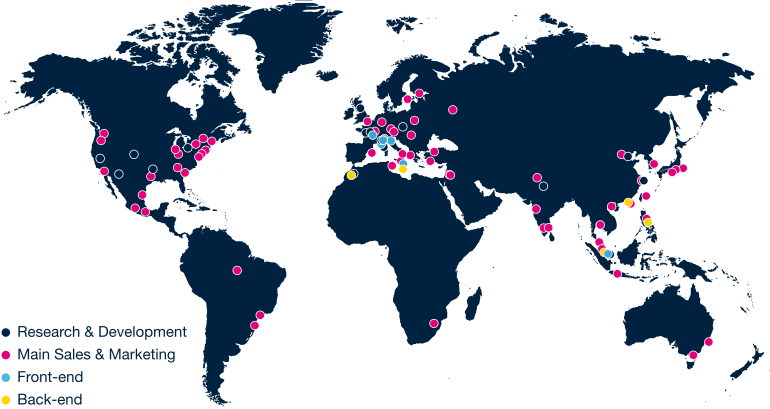
\includegraphics[width=16cm]{st map.png}
  \caption{STMicroelectronics Worldwide Presence}
  \label{fig:map}
\end{figure}

\subsection{ST Tunis}

The STMicroelectronics Tunis site, located in the El Ghazela Technopark, employs over 100 professionals in various fields such as tools, applications, quality, and support functions. The facility is involved in all stages of the microelectronics industry, from initial circuit design to final verification before mass production.

With expertise in both hardware and software, the Tunis center's activities include electronic circuit design, software tool development, application software support, and the electrical validation and verification of new circuits. This diverse skill set allows the center to contribute significantly to ST's global operations.

 \begin{figure}[htp]
  \centering
  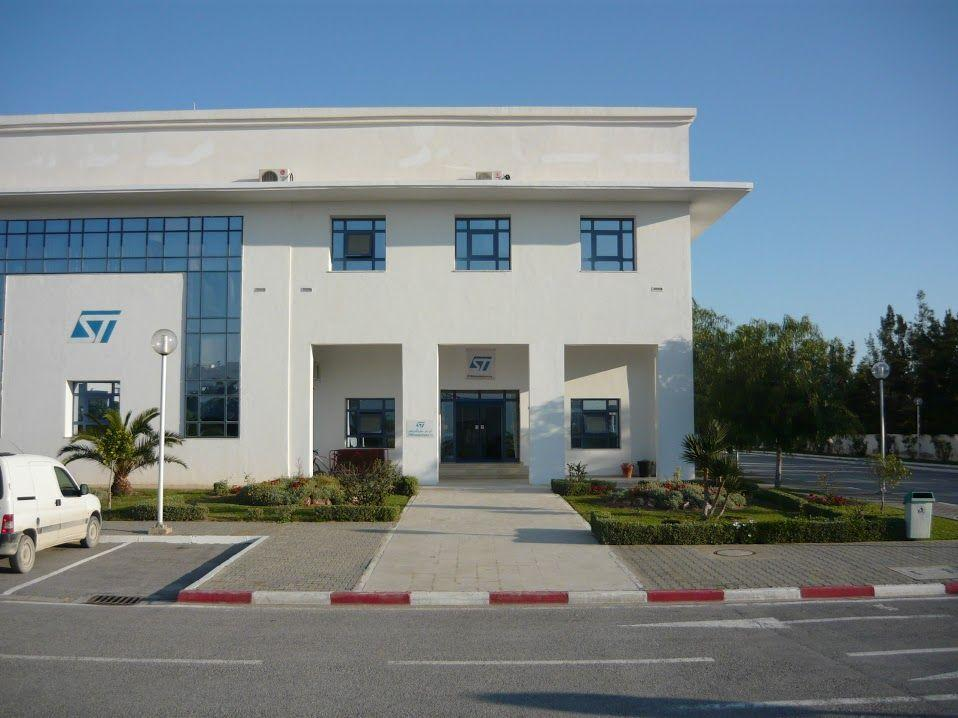
\includegraphics[width=10cm]{stmicroelectronics-tunis-site.jpg}
  \caption{STMicroelectronics Tunis}
  \label{fig:talan_graphe}
\end{figure}


\subsection{ST Support Solutions }
The ST Support Solutions team is dedicated to delivering comprehensive customer support while managing and publishing STM32 product documentation. Their role includes providing in-depth technical support for ST’s tools and products, helping customers troubleshoot problems and optimize their use of these technologies. They ensure the accuracy, clarity, and consistency of all technical documentation, which is regularly updated to reflect the latest developments and innovations. The team is also involved in enhancing and maintaining existing products, as well as defining new products, derivatives, and application references to meet evolving market needs. Additionally, they lead initiatives related to intellectual property applications, offering specific support through the development of application notes, training programs, and other resources that help customers fully understand and utilize ST’s products. This multifaceted approach ensures both customer satisfaction and continuous improvement in the STM32 ecosystem.

\section {Project Context}

Benchmarking microcontrollers is a fundamental step in evaluating their computational capabilities, power efficiency, and suitability for various applications, such as IoT, robotics, or industrial control. Among the many available benchmarks, CoreMark, developed by EEMBC, has become the de facto standard for embedded systems because it provides a well-defined, portable, and reliable performance metric.
STM32 microcontrollers, are widely adopted in the embedded systems industry due to their scalability, rich peripheral set, and performance-to-cost ratio.

The \textbf{CMSIS} initiative, led by Arm, and its Open-CMSIS-Pack ecosystem aim to standardize microcontroller development workflows. Within this ecosystem, Csolution provides a modern, metadata-driven project structure that enables cross-platform builds, device abstraction, and automation. Leveraging Csolution can significantly simplify benchmarking workflows by providing a unified and reproducible project generation and build process.

\section{Problem Statement}
Running CoreMark on STM32 devices traditionally requires manual setup for each device, including:
\begin{itemize}
	\item Creating and configuring individual projects for different STM32 families.
	\item Managing peripheral initialization.
	\item Providing a clock source to Coremark.
	\item Handling different compiler options and toolchains.
	\item Customizing linker scripts manually.
	\item Maintaining multiple project files for IDEs like Keil µVision, IAR EWARM, or others.
\end{itemize}
This manual process is time-consuming, error-prone, and non-scalable, especially when benchmarking a wide range of devices.
There is currently no standardized, automated workflow that allows developers to quickly generate CoreMark-ready projects for different STM32 targets while ensuring consistency and portability.

\section{State of the Art}
The current approaches to running benchmarks on STM32 devices typically rely on:
\begin{itemize}
	\item Vendor-Specific IDEs
		IDEs provide an easy way to manage projects via a graphical interface, they typically provide tools for peripheral configuration, memory management and compiler options.
		They also offer integrated build and debug environments.
	\item Standalone CoreMark Implementations
		EEMBC provides CoreMark source code with minimal reference implementations, it is up to the developer to manually adapt it to the target device, providing startup and initialization code, memory configuration and a clock source.
	\item Custom Build Systems
		Some environments require the use of custom build systems such as CMake and Make, these tools allow the developer to manually manage dependencies, defines and other C/C++ related build configuration.
	\item CMSIS Packs
		CMSIS packs offer a standardized way of packaging drivers, middleware and device specific files, they provide metadata to describe the device's memory and peripheral layout.
\end{itemize}
\section{Critique of Current State of the Art}

While the above methods work, they exhibit several limitations:


\begin{tabularx}{\linewidth}{@{}>{\bfseries}l X X@{}}
	\toprule
	Approach & Advantages & Limitations \\
	\midrule
	Vendor-Specific IDEs & Intuitive GUI, built-in drivers, easy to use & Projects are IDE-specific, hard to automate, poor scalability \\
	\midrule
	Standalone CoreMark & Portable reference code on computers & Significant manual effort for adaptation to each MCU \\
	\midrule
	Custom Build Systems & Flexible, automation-friendly & Requires deep expertise, no standardized metadata integration \\
	\midrule
	CMSIS Packs & Standardized packaging and metadata support & Lack seamless integration with benchmarking and automation \\
	\bottomrule
\end{tabularx}

\section{Proposed Solution}

The proposed solution centers around developing a practical demonstration of the "CryptoEngine," the new cryptography peripheral featured in the STM32XX MCU series. This demo is designed to help users, especially those unfamiliar with cryptography, to understand and utilize the advanced features of this new technology.

To achieve this, the demonstration sets up a secure communication system between two boards: one equipped with the STM32XX MCU using the "CryptoEngine" and the other with an STM32U545 MCU employing existing cryptographic solutions. By highlighting the security enhancements, and ease of use provided by the "CryptoEngine," this demo will serve as a valuable resource for developers, offering a hands-on introduction to the new hardware's capabilities.

\section{Objective}
The primary objective of this project is to develop a practical demonstration that showcases the capabilities of the new "CryptoEngine" in enhancing security and simplifying cryptographic operations. This demonstration will serve as a reference for developers and engineers, providing them with a clear understanding of the new hardware's features and practical applications.

By achieving this objective, the project aims to establish a good starting guide to users of the new "CryptoEngine", which will contribute to the development of more secure and robust cryptographic solutions, thereby enhancing the overall security posture of IoT and connected devices.

\section{Conclusion}

To conclude, this chapter has introduced STMicroelectronics, including its global operations, the ST Tunis site, and the Support Solutions team. We have highlighted the growing importance of security for microcontrollers, especially within the IoT landscape, and identified the existing limitations in the current cryptographic solutions available for STM32 products.

The proposed "CryptoEngine" is designed to address these challenges by providing enhanced security features combined with improved usability. By developing a practical demonstration of this new peripheral, the project aims to offer a comprehensive introduction to its capabilities, thus enabling users to effectively implement and benefit from advanced cryptographic solutions.
